%\documentclass[tikz]{standalone}
%\usepackage{pgfplots}
% the figures style are inspired by \url{https://www.nature.com/articles/nature14122/figures/12}.
% For the use of draw group line, refer to https://tex.stackexchange.com/questions/55554/how-can-i-mix-an-ybar-and-an-ybar-stacked-with-pgfplots
%\begin{document}



% figure a -------------------------------------------------------


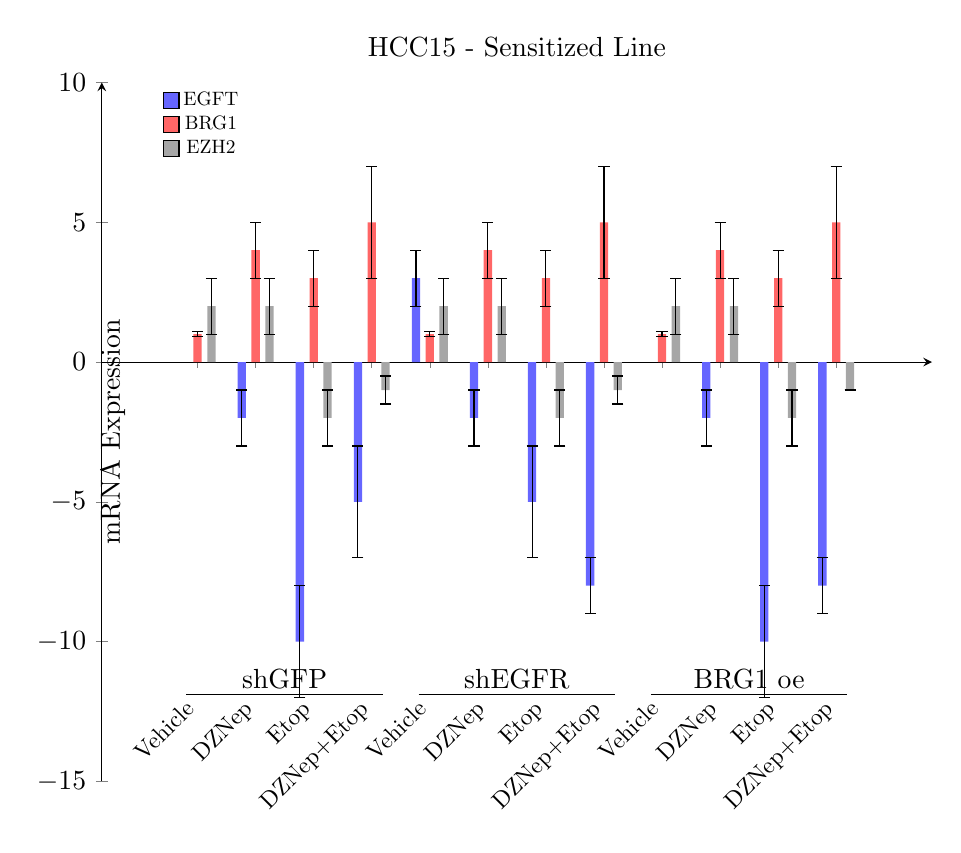
\begin{tikzpicture}
\newcounter{groupcnt}
% draw group line={<group column>}{<group value>}{<group label>}{<vertical offset>}{<line extension>}{<table name>}
\pgfplotsset{
    draw group line/.style n args={6}{
        after end axis/.append code={
            \setcounter{groupcnt}{0}
            \pgfplotstableforeachcolumnelement{#1}\of#6\as\cell{%
                \def\temp{#2}
                \ifx\temp\cell % if current row is in the group
                    \ifnum\thegroupcnt=0
                        \stepcounter{groupcnt}
                        \pgfplotstablegetelem{\pgfplotstablerow}{X}\of#6
                        \coordinate [yshift=#4] (startgroup) at (axis cs:\pgfplotsretval,0);
                    \else
                        \pgfplotstablegetelem{\pgfplotstablerow}{X}\of#6
                        \coordinate [yshift=#4] (endgroup) at (axis cs:\pgfplotsretval,0);
                    \fi
                \else % if we reach the end of current group
                    \ifnum\thegroupcnt=1
                        \setcounter{groupcnt}{0}
                        \draw [
                            shorten >=-#5,
                            shorten <=-#5
                        ] (startgroup) -- node [anchor=base, yshift=0.5ex] {#3} (endgroup);
                    \fi
                \fi
            }% end of for each column element
            \ifnum\thegroupcnt=1 % if we are at the end row
                        \setcounter{groupcnt}{0}
                        \draw [
                            shorten >=-#5,
                            shorten <=-#5
                        ] (startgroup) -- node [anchor=base, yshift=0.5ex] {#3} (endgroup);
            \fi
        }
    }
} % draw group line end -----------------

\pgfplotsset{my error bar/.style={
    error bars/.cd,y dir =both, y explicit,
  }
}

\pgfplotstableread{
X Gp  name EGFR EGFRerr BRG1 BRG1err EZH2 EZH2err
1 shGFP   Vehicle 0 0 1 0.1 2 1
2 shGFP   DZNep -2 1 4 1 2 1
3 shGFP   Etop -10 2 3 1 -2 1
4 shGFP   DZNep+Etop -5 2 5 2 -1 0.5
5 shEGFR  Vehicle 3 1 1 0.1 2 1
6 shEGFR  DZNep -2 1 4 1 2 1
7 shEGFR  Etop -5 2 3 1 -2 1
8 shEGFR  DZNep+Etop -8 1 5 2 -1 0.5
9  BRG1oe Vehicle 0 0 1 0.1 2 1
10 BRG1oe DZNep -2 1 4 1 2 1
11 BRG1oe Etop -10 2 3 1 -2 1
12 BRG1oe DZNep+Etop -8 1 5 2 -1 0.
}{\tabletwo}
\begin{axis}[
    width = \linewidth,
    title={HCC15 - Sensitized Line},
    ybar,
    bar width=3pt,
    axis x line = center, % change the default axis box.
    axis y line = left,
    enlarge x limits=0.15,
    ymin=-15, ymax=10,
    % legned related -------------
    legend image code/.code={
        \draw [#1] (0cm,-0.1cm) rectangle (0.2cm,0.1cm);
    },
    legend style={
        at={(0.18,1)},
        nodes={scale=0.7},
        draw = none     % without box
    },
    ylabel={mRNA Expression},
    % xtick related 
    xtick=data,
    xticklabels from table={\tabletwo}{name},
    xticklabel style={
        rotate=45,xshift=-85,yshift=-85,
        anchor=mid east,
        scale=0.85,
    },
    ylabel style={at={(axis description cs:0.04,0.5)}},
    draw group line={Gp}{shGFP}{shGFP}{-120}{4pt}{\tabletwo},
    draw group line={Gp}{shEGFR}{shEGFR}{-120}{4pt}{\tabletwo},
    draw group line={Gp}{BRG1oe}{BRG1 oe}{-120}{4pt}{\tabletwo},
    ] % end of options of axis environment

% the "!" denotes the intensity
\addplot [draw=none, fill=blue!60,my error bar] table [y=EGFR,y error=EGFRerr] {\tabletwo};
\addplot [draw=none, fill=red!60,my error bar] table [y=BRG1,y error=BRG1err] {\tabletwo};
\addplot [draw=none, fill=gray!70,my error bar] table [y=EZH2,y error=EZH2err] {\tabletwo};

\legend{EGFT,BRG1,EZH2}

\end{axis}
\end{tikzpicture}

%\end{document}